 \ifx\PREAMBLE\undefined
\documentclass{report}
\usepackage[format = hang, font = bf]{caption}
\usepackage{subcaption}
% The following is needed in order to make the code compatible
% with both latex/dvips and pdflatex. Added for using UML generated by MetaUML.
\ifx\pdftexversion\undefined
\usepackage[dvips]{graphicx}
\else
\usepackage[pdftex]{graphicx}
\DeclareGraphicsRule{*}{mps}{*}{}
\fi
\usepackage{array}
\usepackage{amsmath}
\usepackage{amsthm}
\usepackage{mathtools}
\usepackage{boxedminipage}
\usepackage{listings}
\usepackage{multicol}
\usepackage{makecell}%diagonal line in table
\usepackage{float}%allowing forceful figure[H]
\usepackage{xcolor}
\usepackage{mathrsfs}%mathcal
\usepackage{amsfonts}%allowing \mathbb{R}
\usepackage{amssymb}
\usepackage{alltt}
\usepackage{algorithmicx}
\usepackage[chapter]{algorithm} 
%chapter option ensures that algorithms are numbered within each chapter rather than in the whole article
\usepackage[noend]{algpseudocode} %If end if, end procdeure, etc is expected to appear, remove the noend option
\usepackage{xspace}
\usepackage{physics}
\usepackage{color}
\usepackage{tikz}
\usetikzlibrary{shapes,positioning}
\usepackage{url}
\def\UrlBreaks{\do\A\do\B\do\C\do\D\do\E\do\F\do\G\do\H\do\I\do\J\do\K\do\L\do\M\do\N\do\O\do\P\do\Q\do\R\do\S\do\T\do\U\do\V\do\W\do\X\do\Y\do\Z\do\[\do\\\do\]\do\^\do\_\do\`\do\a\do\b\do\c\do\d\do\e\do\f\do\g\do\h\do\i\do\j\do\k\do\l\do\m\do\n\do\o\do\p\do\q\do\r\do\s\do\t\do\u\do\v\do\w\do\x\do\y\do\z\do\0\do\1\do\2\do\3\do\4\do\5\do\6\do\7\do\8\do\9\do\.\do\@\do\\\do\/\do\!\do\_\do\|\do\;\do\>\do\]\do\)\do\,\do\?\do\'\do+\do\=\do\#\do\-}
\usepackage{xr}%allow cross-file references
\usepackage[breaklinks = true]{hyperref}
\lstset{
language = C++, 
showspaces = false,
breaklines = true, 
tabsize = 2, 
numbers = left, 
extendedchars = false, 
basicstyle = {\ttfamily \footnotesize}, 
keywordstyle=\color{blue!70}, 
commentstyle=\color{gray}, 
frame=shadowbox, 
rulesepcolor=\color{red!20!green!20!blue!20}, 
numberstyle={\color[RGB]{0,192,192}}, 
moredelim=[is][\underbar]{_}{_}
}
\mathchardef\myhyphen="2D
% switch-case environment definitions
\algblock{switch}{endswitch} 
\algblock{case}{endcase}
%\algrenewtext{endswitch}{\textbf{end switch}} %If end switch is expected to appear, uncomment this line.
\algtext*{endswitch} % Make end switch disappear
\algtext*{endcase}
\algnewcommand\algorithmicinput{\textbf{Input}}
\algnewcommand\Input{\item[\algorithmicinput]}
\algnewcommand\algorithmicoutput{\textbf{Output}}
\algnewcommand\Output{\item[\algorithmicoutput]}
\algnewcommand\algorithmicinputoutput{\textbf{input and output:}}
\algnewcommand\InputOutput{\item[\algorithmicinputoutput]}
\allowdisplaybreaks
\newtheorem{theorem}{Theorem}
\newtheorem{corollary}[theorem]{Corollary}
\newtheorem{lemma}[theorem]{Lemma}
\newtheorem{definition}{Definition}
\begin{document}
\fi
\chapter{Block Ciphers}
\section{Overview}
Block cipher is a more powerful primitive than stream cipher. As with stream cipher, a block cipher is made up of an encryption algorithm $E$ and a decryption algorithm $D$, both of which take as input a key $k$. Both algorithms take as input $n$ bits, and output $n$ bits. There are two canonical examples of block ciphers:
\begin{description}
\item[3DES]$n$ = 64, $k$ = 168;
\item[AES]$n$ = 128, $k$ = 128/192/256.
\end{description}
A block cipher first expands the key $k$ into $t$ \textbf{round keys} $k_1,\dots,k_t$. Then it uses a \textbf{round function} $R(k,m)$ to encrypt the message by sequentially using the round keys and the encryption result in the previous step: $m_1=R(k_1,m),m_2=R(k_2,m_1),\dots,c=R(k_t,m_{t-1})$. We have $t=48$ for 3DES and $t=10$ for AES-128.

Typically block ciphers are slower than stream ciphers. But block ciphers are capable of completing some tasks that cannot be done efficiently with stream ciphers.

\begin{definition}\textbf{(PRF)}
A \textbf{pseudo random function (PRF)} is a function defined over $(K,X,Y)$:
\[F:K\times X\rightarrow Y\]
such that there exists an efficient algorithm to evaluate $F(k,x)$. 
\end{definition}
\begin{definition}\textbf{(PRP)}
A \textbf{pseudo random permutation (PRP)} is a function defined over $(K,X,X)$:
\[E:K\times X\rightarrow X\]
such that 
\begin{itemize}
\item There exists an efficient deterministic algorithm to evaluate $F(k,x)$;
\item The function $F(k,\cdot)$ is one-to-one, i.e. it's invertible;
\item There exists an efficient inversion algorithm $D(k,y)$.
\end{itemize}
\end{definition}
Let $F:K\times X\rightarrow Y$ be a PRF. Let $Funs[X,Y]$ represent the set of all functions from $X$ to $Y$, and $S_F$ represent the set of $F(k,\cdot)$ with $k\in K$. Obviously $S_F\subseteq Funs[X,Y]$.
\begin{definition}\textbf{(Secure PRFs)}
We call $F$ a \textbf{secure PRF} if a random function from $Funs[X,Y]$ is indistinguishable from a random function from $S_F$.
\end{definition}
From a secure PRF $F:K\times \{0,1\}^n\rightarrow\{0,1\}^n$, we can easily construct a secure PRG $G:K\times\{0,1\}^{nt}$:
\[G(k)=F(k,0)\parallel F(k,1)\parallel\dots\parallel F(k,t).\]
A great property of this PRG is that it is parallelizable. We will prove its correctness later.
\section{Data Encryption Standard (DES)}
In order to specify a block cipher, we need to provide the key expansion mechanism and the round function. DES will be used as an example in this section.
\subsection{Feistel Network}
The core idea behind DES is \textbf{Feistel network}. Its goal is to build an invertible function $F:\{0,1\}^{2n}\rightarrow\{0,1\}^{2n}$ from $n$ arbitrary (not necessarily invertible!) functions $f_1,f_2,\dots,f_d:\{0,1\}^n\rightarrow\{0,1\}^n$. The initial input contains two parts $R_0$ and $L_0$, each $n$ bits. Then we have 
\begin{equation*}\begin{cases}
R_i&=L_{i-1}\oplus f_i(R_0)\\
L_i&=R_{i-1}
\end{cases}\end{equation*}
for $i=1,2,\dots,d$, as shown in Figure \ref{feistel}. $R_d,L_d$ are taken as the output. 
\begin{figure}[ht]
\centering
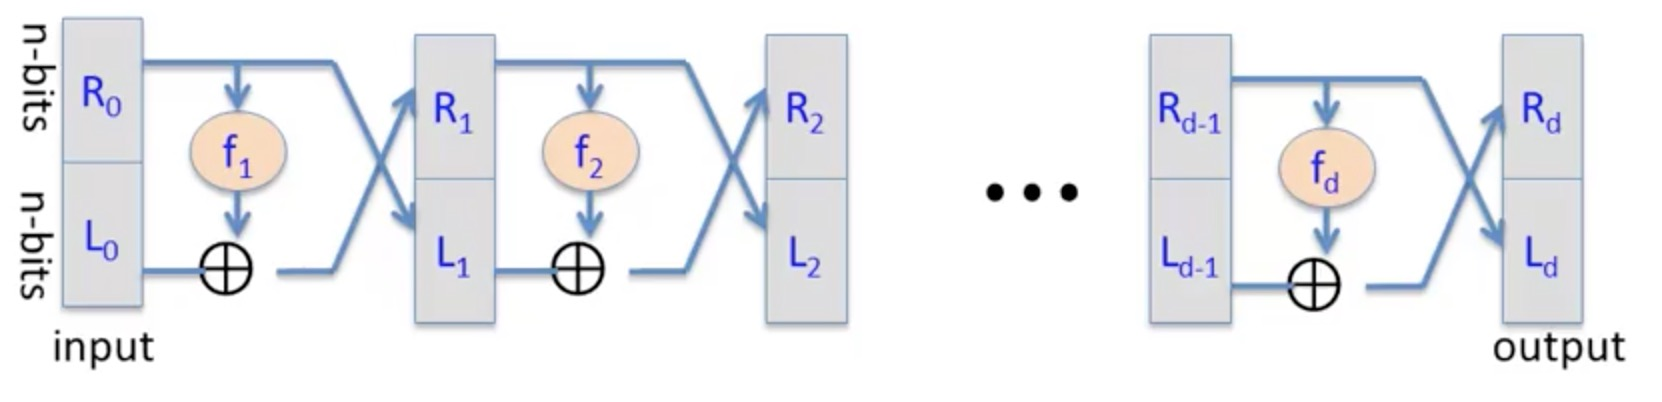
\includegraphics[width=\textwidth]{feistel.jpg}
\caption{Feistel Network}\label{feistel}
\end{figure}

It is easy to construct its inverse:
\begin{equation*}\begin{cases}
R_{i-1}&=L_i\\
L_{i-1}&=f(L_i)\oplus R_i
\end{cases}\end{equation*}
for $i=d,\dots,1$. Feistel network is used in many block ciphers, but not in AES.

The following theorem is important in the theory of DES. 
\begin{theorem}
If $f:K\times\{0,1\}^n\rightarrow\{0,1\}^n$ is a secure PRF, then a 3-round Feistel Network (Figure \ref{3rfeistel}) $F:K^3\times\{0,1\}^{2n}\rightarrow\{0,1\}^{2n}$ is a secure PRP.
\end{theorem}
\begin{figure}[ht]
\centering
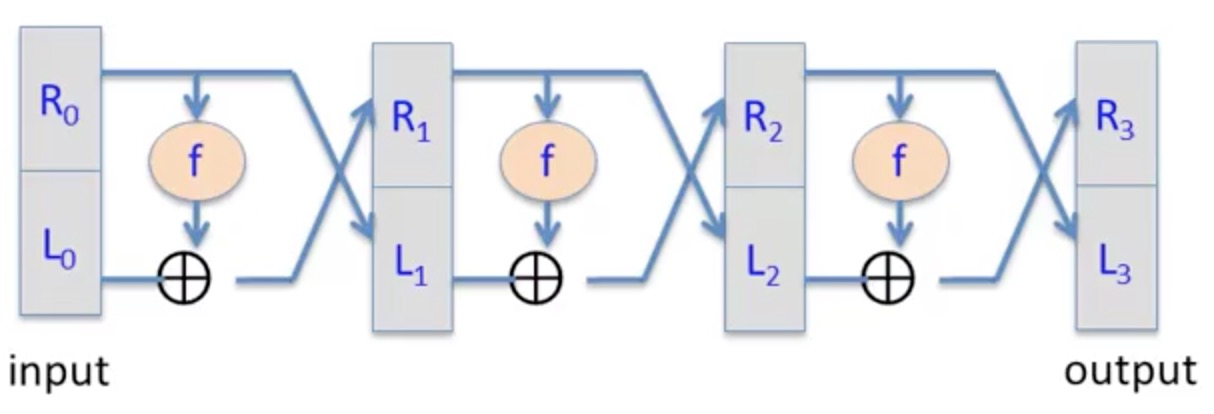
\includegraphics[width=\textwidth]{3rfeistel.jpg}
\caption{3-Round Feistel Network}\label{3rfeistel}
\end{figure}
The theorem means that if we have a secure PRF at hand, we can construct a secure block cipher.

DES is essentially a 16-round Feistel network. It uses 16 functions $F(k_i,x)=f_i(x):\{0,1\}^{32}\rightarrow\{0,1\}^{32},i=1,\dots,16$, as shown in Figure \ref{des}. IP is an initial permutator not for security reason, but required by the standard, and IP$^{-1}$ is its inverse. The Feistel network uses 16 48-bit keys expanded from a 56-bit initial key\footnote{We won't discuss the key expansion.}.
\begin{figure}[ht]
\centering
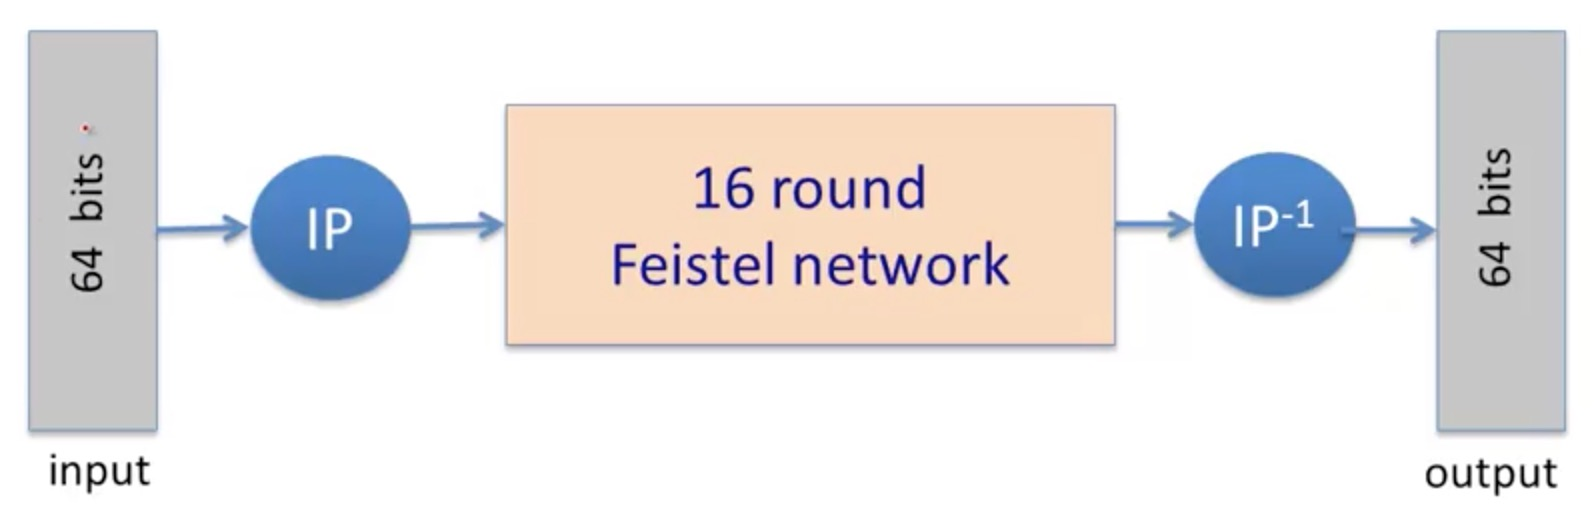
\includegraphics[width=\textwidth]{DES.jpg}
\caption{DES}\label{des}
\end{figure}
\subsection{DES Round Function}
Let's now discuss the round function $F(k_i,x)$. It carries out the following steps.
\begin{enumerate}
\item Pass the 32-bit input $x$ to an expansion box $E$, which expands it to 48 bits $x'$ by simple replications of bits.
\item Compute $x'\oplus k_i$ ($k_i$ is also 48 bits).
\item Break $x'\oplus k_i$ into 8 6-bit groups.
\item Each 6-bit group goes through an $S$ box and gets mapped to 4 bits.
\item Gather the 8 4-bit results and use a $P$ box to permute them into a 32-bit output.  
\end{enumerate}

The $S$ boxes are $\{0,1\}^6\rightarrow\{0,1\}^4$ functions implemented as lookup tables. Figure \ref{sboxeg} is an example.
\begin{figure}[ht]
\centering
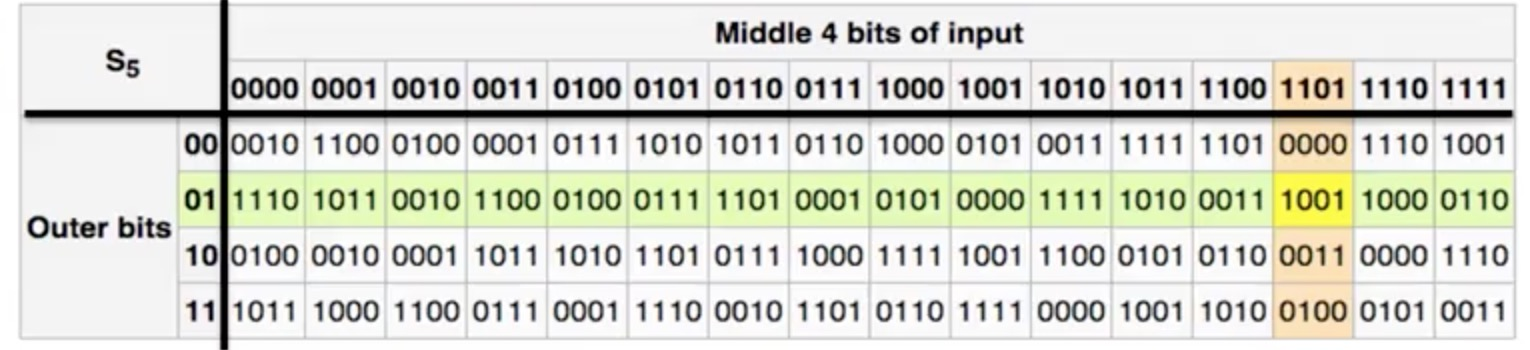
\includegraphics[width=\textwidth]{sboxeg.jpg}
\caption{An Example of $S$ Box}\label{sboxeg}
\end{figure}

The choice of these functions is subtle. For example, linear functions 
\[S_i(\vec{x})=A_i\cdot\vec{x}\pmod 2\]
with $A_i$ being a $4\times 6$ matrix are bad choices. The reason is that we can then find a $64\times 832$ matrix $B$ such that 
\[DES(k,m)=B\cdot\begin{pmatrix}m&k_1&\cdots&k_{16}\end{pmatrix}^{\mathsf{T}}=c,\]
i.e DES as a whole becomes linear. Then we have 
\[DES(k,m_1)\oplus DES(k,m_2)\oplus DES(k,m_3)=DES(k,m_1\oplus m_2\oplus m_3,\]
which is not a property that holds for a random function, and thus makes our DES insecure. What's worse, all round keys can be extracted given 832 $m-c$ pairs.

It has been proven that even choosing the $S$ boxes and $P$ box at random will result in an insecure block cipher. There are a lot of rules limiting the choices in order to guarantee the security of DES.
\section{Attacks on DES}
\subsection{Exhaustive Search Attack}
The goal of an \textbf{exhaustive search attack} is to recover the key $k$ given 3 input-output pairs $m_i,c_i=E(k,m_i),i=1,2,3.$ We use ``the'' key because the following lemma convinces us of its uniqueness.
\begin{lemma}
Suppose DES is an \textbf{ideal cipher}\footnote{This is idealized, not the actual situation}, i.e. DES is a collection of $2^{56}$ random invertible functions 
\[\pi_i:\{0,1\}^{64}\rightarrow\{0,1\}^{64},i=1,\dots,2^{56}.\]
Then $\forall m,c$, 
\[Pr(\text{at most one key s.t. $c=DES(k,m)$})\geq 1-\frac{1}{256}\approx 99.5\%.\]
\end{lemma}
\begin{proof}
\begin{align*}
&Pr(\exists k'\neq k\:s.t.\:c=DES(k,m)=DES(k',m))\\
\leq&\sum\limits_{k'}Pr(DES(k',m)=DES(k,m))\\
=&2^{56}\cdot\frac{1}{2^{64}}=\frac{1}{256}
\end{align*}
\end{proof}
This fact makes it possible to find the $k$ with brute force search with only one $m-c$ pair. It is not that difficult to use modern computers to do this with a 56-bit cipher, so 56-bit DES ciphers should no longer be used. 

There are ways to enhance the security of DES. 
\subsubsection{3DES}
Let $E:K\times M\rightarrow M$ be a 56-bit DES cipher. The define a 3DES cipher $3E:K^{3}\times M\rightarrow M$ as 
\[3E((k_1,k_2,k_3),m)=E(k_1,D(k_2,E(k_3,m))).\]
3DES has the key size of $56\times 3=168$. It is safer than DES, but it is also 3 times slower. We use E-D-E instead of E-E-E in order to be able to produce DES result with $k_1=k_2=k_3$.

The reason to use 3DES instead of 2DES is that 2DES is breakable with less time than it appears to need, making it insecure. Define 
\[2E((k_1,k_2,k_3),m)=E(k_1,E(k_2,m)).\]
Given a $m-c$ pair, we have 
$E(k_1,E(k_2,m))=c$, therefore $D(k_1,c)=E(k_2,m)$, which inspires us of a new way to break the cipher, namely the meet-in-the-middle attack. 

First we calculate $E(k_i,m)$ for all $2^{56}$ possible keys and save them in a table. Then we sort the table according to the value of $E(k_i,m)$. Finally for each possible $k_i$, we calculate $D(k_i,c)$ and search for it in the table. Building and sorting the table takes $2^{56}\log(2^56)$ time. Searching takes another $2^56\log(2^{56})$ time. In total the time consumption is smaller than $2^63\ll 2^112$, making 2DES insecure.

The same strategy can be used to break 3DES in $2^{118}$ time:
\[2^{56}\log(2^{56})+2^{56\times 2}\log(2^{56})=2^{118}.\]
\subsubsection{DESX}
Define DESX cipher $EX:K^{3}\times M\rightarrow M$ as 
\[EX((k_1,k_2,k_3),m)=k_1\oplus E(k_2,k_3\oplus m).\]
It has a key length of 64+56+64=184. A meet-in-the-middle attack takes $2^{120}$ time: using $k_1\oplus c=E(k_2,k_3\oplus m)$, the time consumption is 
\[2^{56+64}\log(2^{56+64})+2^{64}\log(2^{56+64})=2^{120}.\]

Nonetheless, if only one XOR is used, i.e. $k_1$ or $k_3$ is not used, the cipher will be no securer than DES.
\subsection{Side Channel Attacks}
An attacker can obtain the key by precisely measuring the time or power consumption of encryption/decryption. If the cipher is run in one of the cores of a multi-core processor, an attacker can obtain the key by counting the number of cache misses in the shared cache. 
\subsection{Fault Attack}
An error in the last round can expose the secret key. Thus the correctness of the algorithm needs to be guaranteed, which serves as a strong reason for us not to attempt to implement cryptography primitives.
\subsection{Linear/Differential Attacks}
The goal is to recover the key in less than $2^{56}$ time when given many $m-c$ pairs. Suppose for random $k,m$, 
\[Pr((m[i_1]\oplus\cdots\oplus m[i_r])\oplus(c[j_1]\oplus\cdots\oplus c[j_r]) = k[l_1]\oplus\cdots\oplus k[l_r])=\frac{1}{2}+\epsilon\]
holds for some non-zero $\epsilon$, in which $m[i_1]\dots m[i_r]$ is a subset of the message bits, $c[j_1]\dots c[j_r]$ is a subset of the cipher text bits, and $k[l_1]\dots k[l_r]$ is a subset of the key bits, then we have the following theorem.
\begin{theorem}
Given $\frac{1}{\epsilon^2}$ random $m-c$ pairs, then we have
\[k[l_1]\oplus\cdots\oplus k[l_r]=mode((m[i_1]\oplus\cdots\oplus m[i_r])\oplus(c[j_1]\oplus\cdots\oplus c[j_r]))\]
with a probability $\geq 97.7\%$.
\end{theorem}
Mode is the statistical mode: element with maximum frequency. 

For DES, we have $\epsilon=\frac{1}{2^{21}}$. With $2^{42}$ $m-c$ pairs we can find 14 key bits in time $2^{42}$. Then we can do a brute force search for the remaining bits in $2^{42}$ time, thus the overall attack time is $2^{43}\ll 2^{56}$. 

This is another reason against implementing our own ciphers: a little bias of the cipher leads to an easy attack.
\subsection{Quantum Attacks}
Consider a generic problem: given $f:X\rightarrow\{0,1\}$ that is a function evaluating to 0 most of the time, try to find $x\in X$ s.t. $f(x)=1$. On a classical computer, the best generic algorithm takes $O(\lvert X\rvert)$ time. A quantum on the contrary can solve the problem in $O(\sqrt{\lvert X\rvert})$ time.

To attack a block cipher, we can use the function
\begin{equation*}
f(k)=\begin{cases}
1&if\:E(k,m)=c\\
0&otherwise
\end{cases}\end{equation*}
This means that a quantum search algorithm can find the key in $O(\sqrt{\lvert K\rvert})$ time. For DES this means $2^{28}$ time. 
\ifx\PREAMBLE\undefined
\end{document}
\fi